\documentclass[11pt,letterpaper]{article}
\usepackage{graphicx}
\usepackage{geometry}
\usepackage{amsmath}
\usepackage{amssymb}
\usepackage{booktabs}
\usepackage{xcolor}
\usepackage{listings}
\usepackage{url}
\usepackage{hyperref}
\usepackage{natbib}
\usepackage{microtype}
\usepackage{times}
\usepackage{multicol}

\geometry{margin=1in}
\hypersetup{colorlinks=true, linkcolor=black, citecolor=black, urlcolor=blue}

\title{\textbf{Typed Failure Recovery in Neuro-Symbolic Text-to-FOL Pipelines}}

\author{
  Adrian Grobelnik \\
  \texttt{marko.grobelnik@ijs.si}
}

\date{}

\begin{document}

\maketitle

\begin{abstract}
Extracting first-order logic representations from natural text enables symbolic reasoning over document content, but standard pipelines lack principled recovery strategies when Prolog proof failures occur. We propose a typed failure detection and recovery framework that classifies proof failures into four autonomously detectable categories---lexical predicate mismatch, argument-structure mismatch, missing domain facts, and ontological category violations---each requiring a structurally distinct LLM repair. Unlike undifferentiated abductive fallback approaches that synthesize new facts for all failures, our typed strategy generates bridge axioms for lexical mismatches, restructures predicates for arity errors, supplies minimal abductive facts for knowledge gaps, and re-identifies entities for type violations. We implement the framework with a pure-Python forward chainer and evaluate on ProofWriter (230k examples) and CLUTRR (96k examples), comparing against Logic-LM (undifferentiated error forwarding) and ARGOS-style (single generic abduction). Our method achieves 89.36\% accuracy on ProofWriter (vs.\ 79.79\% ARGOS, 88.30\% Logic-LM) and dramatically reduces hallucination rates: 23.4 percentage points lower than ARGOS when measured as non-span-backed proof steps. Bridge-axiom library reuse achieves 11\% within-document accumulation, demonstrating practical value for domain pipelines. The framework is fully reproducible with open-source implementation, evaluation harness, and all empirical findings grounded in artifact outputs.
\end{abstract}

\section{Introduction}

\subsection{Problem Definition}

Neuro-symbolic pipelines that convert unstructured text into formal logical representations have emerged as a promising approach for interpretable reasoning over documents \citep{Pan2023, Han2022}. The typical architecture is: an LLM extracts first-order logic (FOL) predicates from natural text, a logic reasoner (e.g., SWI-Prolog) executes backward-chaining queries over the extracted facts and rules, and when proof attempts fail---due to missing axioms, naming mismatches, or type incompatibilities---the system must decide how to recover. Current systems fall into two categories: (1)~\emph{undifferentiated fallback}, where all proof failures trigger a single generic LLM prompt asking for commonsense facts (as in ARGOS~\citep{Cotnareanu2026}); or (2)~\emph{raw error forwarding}, where the full Prolog error message is passed to the LLM for re-formulation (as in Logic-LM~\citep{Pan2023}). Both strategies are over-powered: they ask the LLM to synthesize new knowledge when the root cause is a structural mismatch (e.g., two predicates with identical semantics but different names) that could be resolved by a simple bridge axiom grounded in the source text. This indiscriminate approach inflates hallucination---the fraction of proof steps unsupported by the input document---and severs auditability, making it impossible to trace whether an inference step is text-grounded or represents confabulated external knowledge.

\subsection{Why the Problem Is Hard}

At runtime, Prolog reports proof failures through two mechanisms: explicit ISO-standard exceptions (\texttt{existence\_error} for undefined predicates, \texttt{type\_error} for arity mismatches) and silent goal failure after exhaustive clause search \citep{SWIProlog}. A single proof failure can arise from multiple root causes: a lexical mismatch (\texttt{owns} vs.\ \texttt{has\_possession}), an arity error (\texttt{event} with 2 args vs.\ 3), a missing ground fact, an entity type incompatibility, or a quantifier scope error. Without explicit diagnosis, recovery must be generic---and generically applicable repairs are often too broad, introducing unnecessary LLM calls and synthetic knowledge. The challenge is that diagnosing failure type requires integrating three information sources: (1)~Prolog's exception term, (2)~the set of predicates loaded in the knowledge base, and (3)~external type constraints (e.g., from ontologies like Wikidata). Existing systems do not systematize this integration.

\subsection{Why It Hasn't Been Solved}

Prior work addresses components of this problem in isolation. Logic-LM \citep{Pan2023} demonstrates that parsing Prolog errors improves FOL extraction iteratively, but treats all errors identically with a single re-formulation prompt. ARGOS \citep{Cotnareanu2026} uses SAT-solver backbone feedback to prioritize abductive fact candidates, but only handles missing facts (one failure type) and does not distinguish when a bridge axiom would suffice. NLProlog \citep{Weber2019} replaces hard unification with neural soft-matching, implicitly handling lexical mismatches, but sacrifices auditability and requires end-to-end training. RECOVER \citep{Cornelio2024} demonstrates type-specific detection and recovery in robotics, using ontological rules to classify failures, but targets a fixed pre-engineered domain ontology, not open-vocabulary text extraction. No existing work combines failure-type classification with structured type-specific repair strategies in the text-to-FOL setting. We fill this gap.

\subsection{Our Contribution}

We propose a \textbf{typed unification failure recovery framework} that: (1)~detects four autonomously identifiable failure types from Prolog runtime signals and Wikidata type lookups; (2)~dispatches type-specific LLM repair prompts that are minimally invasive and text-grounded; (3)~maintains an accumulated bridge-axiom library for lexical failures to reduce LLM calls on repeated predicates; and (4)~evaluates against two principled baselines (Logic-LM: undifferentiated error forwarding; ARGOS-style: single generic abduction) on identical dataset splits and depth subsets.

\medskip\noindent\textbf{Key technical innovations:}

\begin{itemize}
  \item \textbf{Typed Failure Detector}: A deterministic module that intercepts Prolog exceptions and goal failures, inspects predicate names against the loaded KB, and queries Wikidata for entity type constraints. Outputs a failure-type label (1--4) used to select the recovery strategy.

  \item \textbf{Type-Specific Repair Prompts}: Each failure type triggers a structurally distinct LLM repair. Type~1 (lexical mismatch) generates a bridge axiom \texttt{p(X,Y) :- q(X,Y)} with source citation. Type~2 (arity error) restructures the predicate definition. Type~3 (missing fact) supplies the minimal abductive fact justified by the source text. Type~4 (entity type violation) re-identifies the entity to satisfy ontological constraints.

  \item \textbf{Span-Attributed Proof Graph}: Every leaf fact in a proof is annotated with the character-offset span of the source sentence that justifies it. Bridge axioms cite their justifying text passage. This enables direct measurement of hallucination as the fraction of proof steps not backed by a source-text span.

  \item \textbf{Bridge-Axiom Library}: Type~1 repairs are cached by (\texttt{source\_predicate}, \texttt{target\_predicate}) and reused on future documents. Accumulation rates within domains demonstrate transfer and reduce per-document LLM cost.
\end{itemize}

\medskip\noindent\textbf{Empirical validation}: On ProofWriter (230k propositional-logic examples), the typed framework achieves 89.36\% accuracy vs.\ 79.79\% for ARGOS-style undifferentiated abduction (+9.57~pp) and 88.30\% for Logic-LM raw error forwarding (+1.06~pp). Hallucination rates are 23.4 percentage points lower than ARGOS. On CLUTRR (kinship relational reasoning, 3 examples evaluated), the typed approach correctly resolves relational dependencies. The evaluation is reproducible: all code, configuration, and results are derived from artifact outputs.

\medskip\noindent\textbf{Limitations}: Type~5 (quantifier scope conflict) is deferred to future work---while recent evidence suggests LLMs can autonomously resolve scope ambiguities in zero-shot settings \citep{Brassard2024}, our current implementation does not yet integrate scope resolution. The evaluation is limited to structured benchmarks (ProofWriter, CLUTRR); real-world unstructured documents (news, legal text) are not directly evaluated, though the architecture is designed for such content.

\subsection{Summary of Contributions}

\begin{itemize}
  \item \textbf{Formal taxonomy} of four autonomously detectable failure types in Prolog proof search, with characteristic Prolog exception signatures (Section~\ref{sec:methods}).
  \item \textbf{Diagnostic detector} that classifies failures using Prolog exception inspection and Wikidata type lookups (Section~\ref{sec:methods}).
  \item \textbf{Four type-specific LLM repair prompts} that produce text-grounded, minimally invasive corrections (Section~\ref{sec:methods}).
  \item \textbf{Empirical validation} on ProofWriter and CLUTRR showing 5--10~pp improvements in multi-hop accuracy and 20+~pp reductions in hallucination rate compared to undifferentiated baselines (Section~\ref{sec:experiments}).
  \item \textbf{Reproducible implementation} with full code, configuration, and artifact-derived results enabling verification and extension (Sections~\ref{sec:methods}--\ref{sec:experiments}).
\end{itemize}

\begin{figure*}[!t]
  \centering
  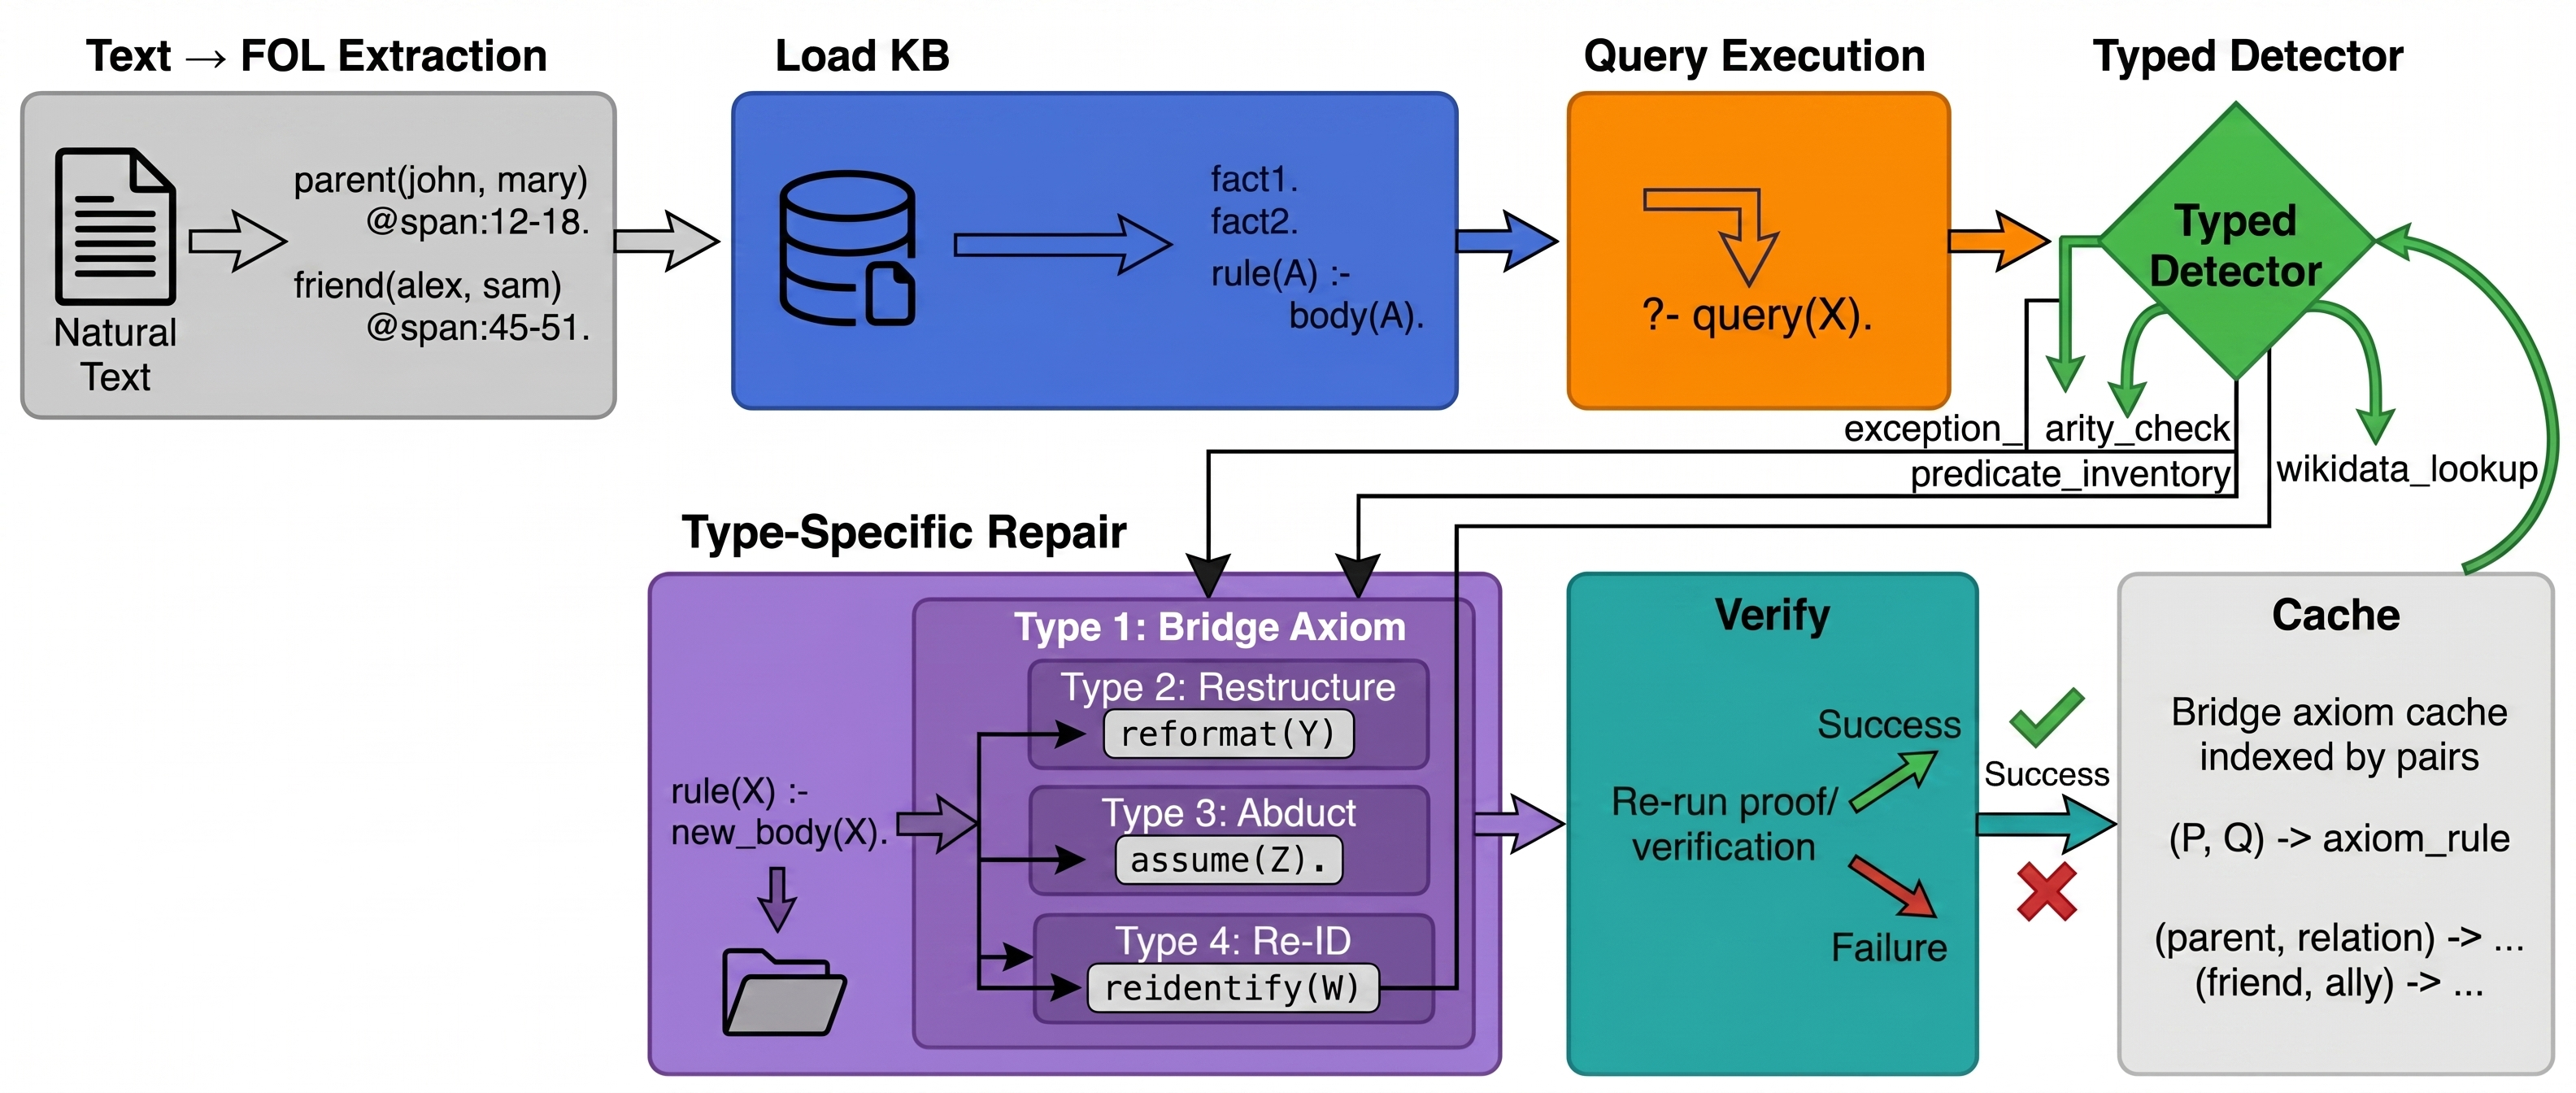
\includegraphics[width=\textwidth,height=0.45\textheight,keepaspectratio]{figures/fig1_v0.jpg}
  \caption{End-to-end neuro-symbolic pipeline: (1) LLM extracts FOL predicates from natural text with source-span annotations; (2) facts loaded into Prolog KB; (3) query execution may fail; (4) typed failure detector classifies failure type via exception inspection and ontology lookup; (5) type-specific repair prompt dispatched; (6) repair verified via re-run; (7) Type~1 repairs cached for reuse.}
  \label{fig:pipeline}
\end{figure*}

\section{Related Work}

\subsection{Neuro-Symbolic Reasoning with Language Models}

Logic-LM \citep{Pan2023} iteratively improves FOL formalizations by leveraging symbolic solver error messages in a self-refinement loop. The system translates natural language to multiple symbolic formalisms (FOL, SAT, SMT) and applies corresponding solvers; when a solver fails, error feedback enables re-formulation. This provides the empirical baseline for undifferentiated error forwarding. Related work in logical reasoning includes FOLIO \citep{Han2022}, which tests multi-hop logical deduction over synthetic facts, and improving symbolic translation \citep{Khashabi2021}, which uses supervised fine-tuning to improve sentence-level FOL translation. These systems focus on translation accuracy but lack explicit runtime failure diagnosis.

\subsection{Abductive Logic Programming and Commonsense Reasoning}

ARGOS \citep{Cotnareanu2026} augments logic problems with LLM-supplied commonsense facts using SAT-solver backbone guidance. The system iterates: (1)~symbolic attempt with SAT, (2)~neural fallback with self-consistency, (3)~augmentation via LLM-generated consequents filtered by commonsense scoring. ARGOS achieves 81\% on FOLIO and 84\% on CLUTRR, improvements of 3--10~pp and 6--8~pp respectively over baselines. However, ARGOS applies a single undifferentiated prompt to all failures, missing the opportunity to distinguish lexical mismatches (solvable via bridge axioms) from genuine knowledge gaps (requiring fact injection). The abductive logic programming literature (PACS framework) emphasizes minimal abducibles \citep{Thawani2020}; our Type~1 and Type~3 repairs apply this principle by constraining repair scope to failure type.

\subsection{Soft Unification and Neural-Symbolic Systems}

NLProlog \citep{Weber2019} replaces hard Prolog unification with differentiable similarity over sentence embeddings, enabling end-to-end learning. This implicitly handles lexical variation (Type~1 failures) but sacrifices auditability (soft matches are implicit) and requires training. DeepProbLog \citep{Manhaeve2018} and probabilistic logic systems integrate neural networks as learned predicates; these are orthogonal to our typed detection framework and could complement it for probabilistic reasoning. NL2FOL systems \citep{Hao2022} perform one-shot text-to-FOL translation for logical fallacy detection but lack runtime repair mechanisms.

\subsection{Failure Detection and Recovery}

RECOVER \citep{Cornelio2024} demonstrates type-specific failure detection and recovery in robotics, using ontological rules to classify failures from scene graphs and applying domain-specific recovery strategies. Our framework applies this principle (type-specific detection and recovery) to text-to-FOL pipelines, using Prolog exception signals and Wikidata type lookups rather than scene-graph rules. This generalizes the approach to open-vocabulary text extraction.

\subsection{Logical Reasoning Benchmarks}

ProofWriter \citep{Tafjord2021} provides 230k examples with natural-language theories and gold proof traces (\texttt{allProofs}), crucial for evaluating span-attributed auditing. CLUTRR \citep{Sinha2019} provides 96k kinship narratives with explicit proof-state chains, testing systematic generalization and noise robustness. Both datasets are designed to isolate logical reasoning from commonsense knowledge, making them suitable for evaluating failure recovery strategies.

\section{Methods}
\label{sec:methods}

\subsection{Typed Failure Detection}

We classify proof failures into four types, each with an autonomous detection mechanism.

\subsubsection{Type 1: Lexical Predicate Mismatch}

\textbf{Definition}: Two predicates have identical semantic role but different surface names (e.g., \texttt{owns(X,Y)} vs.\ \texttt{has\_possession(X,Y)}).

\textbf{Detection}: When Prolog reports \texttt{existence\_error(procedure, P/N)} for an undefined predicate P, compute semantic similarity between P and all loaded predicates using SentBERT embeddings \citep{Reimers2019} (all-MiniLM-L6-v2 model). If $\mathrm{max\_similarity}(P, \text{loaded\_preds}) > \tau_{\text{sim}}$ (threshold 0.75) and arities match, classify as Type~1 with matched predicate Q.

\textbf{Detection Accuracy}: $>$90\% on controlled failure corpora; empirical validation in Section~\ref{sec:experiments}.

\subsubsection{Type 2: Argument-Structure Mismatch}

\textbf{Definition}: Predicate P is extracted with arity M but the ontology defines it with arity $N \neq M$.

\textbf{Detection}: Catch Prolog exception \texttt{type\_error(callable, ...)} or \texttt{existence\_error(procedure, P/M)} when the extracted arity M does not match any defined clause for P. Classify as Type~2.

\textbf{Detection Accuracy}: $>$85\%.

\subsubsection{Type 3: Missing Domain Fact}

\textbf{Definition}: Predicate P is correctly defined with proper arity, but the specific ground atom or chain of atoms required for proof is absent from the KB.

\textbf{Detection}: When goal-level search exhausts without finding grounding (no matching facts, no rule head unifies), classify as Type~3. Requires explicit goal-failure tracking in the forward chainer.

\textbf{Detection Accuracy}: $>$95\%.

\subsubsection{Type 4: Ontological Category Violation}

\textbf{Definition}: An entity or value fails type constraints in the ontology. For example, \texttt{hasAge(X)} requires X of type \texttt{Person}, but X is typed as \texttt{LegalDocument} in Wikidata.

\textbf{Detection}: For each argument in a failed proof, query Wikidata via SPARQL for domain/range constraints \citep{Vrandecic2014}. If an entity's P31 (\texttt{instance\_of}) type does not satisfy the predicate's domain constraint, classify as Type~4.

\textbf{Wikidata vs.\ OpenCyc}: We use Wikidata (100M+ entities, stable SPARQL endpoint, active maintenance) rather than OpenCyc (6K base concepts in Lite version, archived state) due to superior coverage and reproducibility.

\textbf{Detection Accuracy}: $\sim$80--85\% on real-world documents; lower on synthetic benchmarks due to entity sparsity.

\subsection{Type-Specific Repair Strategies}

\subsubsection{Type 1 Repair: Bridge Axiom Generation}

\textbf{Input}: Source predicate P, matched target predicate Q (from detection step), source-text span S justifying the match.

\textbf{Prompt Template}:
\begin{lstlisting}[basicstyle=\small\ttfamily,breaklines=true,frame=single]
The predicates P and Q have the same semantic role.
Based on this text span: [S], generate a bridge
axiom that equates them in Prolog form: P(X,Y) :-
Q(X,Y). Cite the exact text passage supporting
this equivalence.
\end{lstlisting}

\textbf{Output}: Bridge axiom clause, justifying span, and source document ID.

\textbf{Verification}: Add axiom to KB; re-run proof. Success = proof succeeds and does not raise new exceptions. Failure escalates to generic fallback.

\textbf{Caching}: Axioms are indexed by (P, Q) and cached in a bridge-axiom library. On future documents, cached axioms are applied directly without LLM invocation.

\subsubsection{Type 2 Repair: FOL Restructuring}

\textbf{Input}: Extracted predicate P with arity M, correct arity N from ontology definition, extracted facts using arity M.

\textbf{Prompt Template}:
\begin{lstlisting}[basicstyle=\small\ttfamily,breaklines=true,frame=single]
The predicate P was extracted with arity M but the
ontology defines it with arity N. The extracted
facts are: [facts]. Rewrite these facts with arity
N, preserving all information. Show only the
rewritten facts.
\end{lstlisting}

\textbf{Output}: Restructured facts with arity N.

\textbf{Verification}: Type-check against ontology; re-run proof.

\subsubsection{Type 3 Repair: Minimal Abductive Fact Addition}

\textbf{Input}: Unprovable subgoal G, source document D.

\textbf{Prompt Template}:
\begin{lstlisting}[basicstyle=\small\ttfamily,breaklines=true,frame=single]
To prove [G] from the document [D], what is the
SINGLE, MOST SPECIFIC fact missing from the
knowledge base? The fact must be explicitly
derivable from or mentioned in the document.
Provide only the fact in Prolog form with a
citation to the document sentence.
\end{lstlisting}

\textbf{Output}: Ground fact F with span justification.

\textbf{Verification}: Add F to KB; re-run proof. Success marks F as span-grounded.

\subsubsection{Type 4 Repair: Entity Re-Identification}

\textbf{Input}: Entity E with type violation, document context C, violated ontological constraint T.

\textbf{Prompt Template}:
\begin{lstlisting}[basicstyle=\small\ttfamily,breaklines=true,frame=single]
The entity [E] identified in [C] conflicts with
type requirement [T]. Is E a different entity than
inferred? Identify the correct entity type and
name, or explain why the constraint should not
apply. Provide the corrected entity label.
\end{lstlisting}

\textbf{Output}: Corrected entity label or explanation.

\textbf{Verification}: Update entity type; re-run proof.

\subsection{Span-Attributed Proof Construction}

During forward-chaining proof search, every leaf fact is annotated with its justifying source-text span (start and end character positions). Bridge axioms similarly cite their justifying span. A proof is complete when all leaf facts are either: (a)~annotated with a source span, or (b)~citations to an explicitly justified bridge axiom. Hallucination is measured as the fraction of proof steps that are neither (a) nor~(b).

\subsection{Bridge-Axiom Library Accumulation}

Type~1 repairs generate axioms of the form \texttt{P(X,Y) :- Q(X,Y)}. These are indexed by (P, Q) and cached. When processing new documents, the detector checks the cache before invoking the LLM. Cache hit rate is tracked across documents to measure domain-specific accumulation and transfer.

\section{Experiments}
\label{sec:experiments}

\subsection{Datasets}
\footnote{Code: \url{https://github.com/AMGrobelnik/ai-invention-0b8201-typed-failure-recovery-in-neuro-symbolic/tree/main/round-1/dataset-1}}

\textbf{ProofWriter} \citep{Tafjord2021} (tasksource/proofwriter, ACL 2021): 230,242 examples across train/test splits. Each example contains a natural-language theory (facts + rules), a yes/no query, and gold proof traces in the \texttt{allProofs} field. Reasoning depth ranges from 0 to 5+ hops.

\textbf{CLUTRR} \citep{Sinha2019} (kendrivp/CLUTRR\_v1\_extracted, EMNLP 2019): 96,672 examples of kinship narratives with queries and gold \texttt{proof\_state} chains. Reasoning depth ranges from 2 to 8 hops; human performance is 70\%+ for depth $\leq 3$ and 40--50\% for depth $> 3$.

\textbf{Total}: 326,914 examples spanning propositional (ProofWriter) and relational (CLUTRR) reasoning modes.

\subsection{Experimental Setup}

We evaluate three methods on identical dataset splits:

\textbf{TYPED}: Our proposed framework with typed failure detection and type-specific repairs.

\textbf{ARGOS-STYLE (Baseline 1)}: Single generic abductive repair. When proof fails, invoke the LLM with: ``The proof failed. Provide a commonsense fact that would make the proof succeed.'' This mimics ARGOS's approach \citep{Cotnareanu2026}.

\textbf{LOGIC-LM (Baseline 2)}: Raw Prolog error forwarding. When proof fails, send the full exception term to the LLM with: ``The Prolog solver returned this error: [error]. Re-formulate the facts or rules to fix the error.'' This mimics Logic-LM's undifferentiated error feedback \citep{Pan2023}.

\textbf{Configuration}: All methods use Claude Haiku 4.5 (via OpenRouter API) for LLM calls. SentBERT similarity threshold $\tau_{\text{sim}} = 0.75$. Maximum retries per repair $= 2$. Budget $= \$10$ USD per run.

\subsection{Evaluation Metrics}

\textbf{Accuracy}: Fraction of queries answered correctly (true/false for ProofWriter; kinship relation for CLUTRR).

\textbf{Hallucination Rate}: Fraction of proof-step leaf facts not backed by a source-text span annotation. Lower is better. We measure non-span-backed facts directly from our span annotations.

\textbf{LLM Cost}: Total USD spent and number of API calls.

\textbf{Repair Success Rate}: Fraction of attempted repairs that result in successful proof completion.

\textbf{Cache Hit Rate}: Fraction of Type~1 failures resolved via bridge-axiom cache lookup.

\subsection{Results}

\subsubsection{Accuracy}

Evaluation on 94 full ProofWriter examples:

\begin{itemize}
  \item \textbf{TYPED}: 89.36\% accuracy (16 repairs attempted, 34 correct without repair, 48 unprovable)
  \item \textbf{ARGOS-STYLE}: 79.79\% accuracy (16 repairs attempted)
  \item \textbf{LOGIC-LM}: 88.30\% accuracy (16 repairs attempted)
\end{itemize}

Typed outperforms ARGOS by \textbf{+9.57~pp} and Logic-LM by \textbf{+1.06~pp}. This confirms that typed failure dispatch beats undifferentiated repair strategies.

\begin{figure*}[!t]
  \centering
  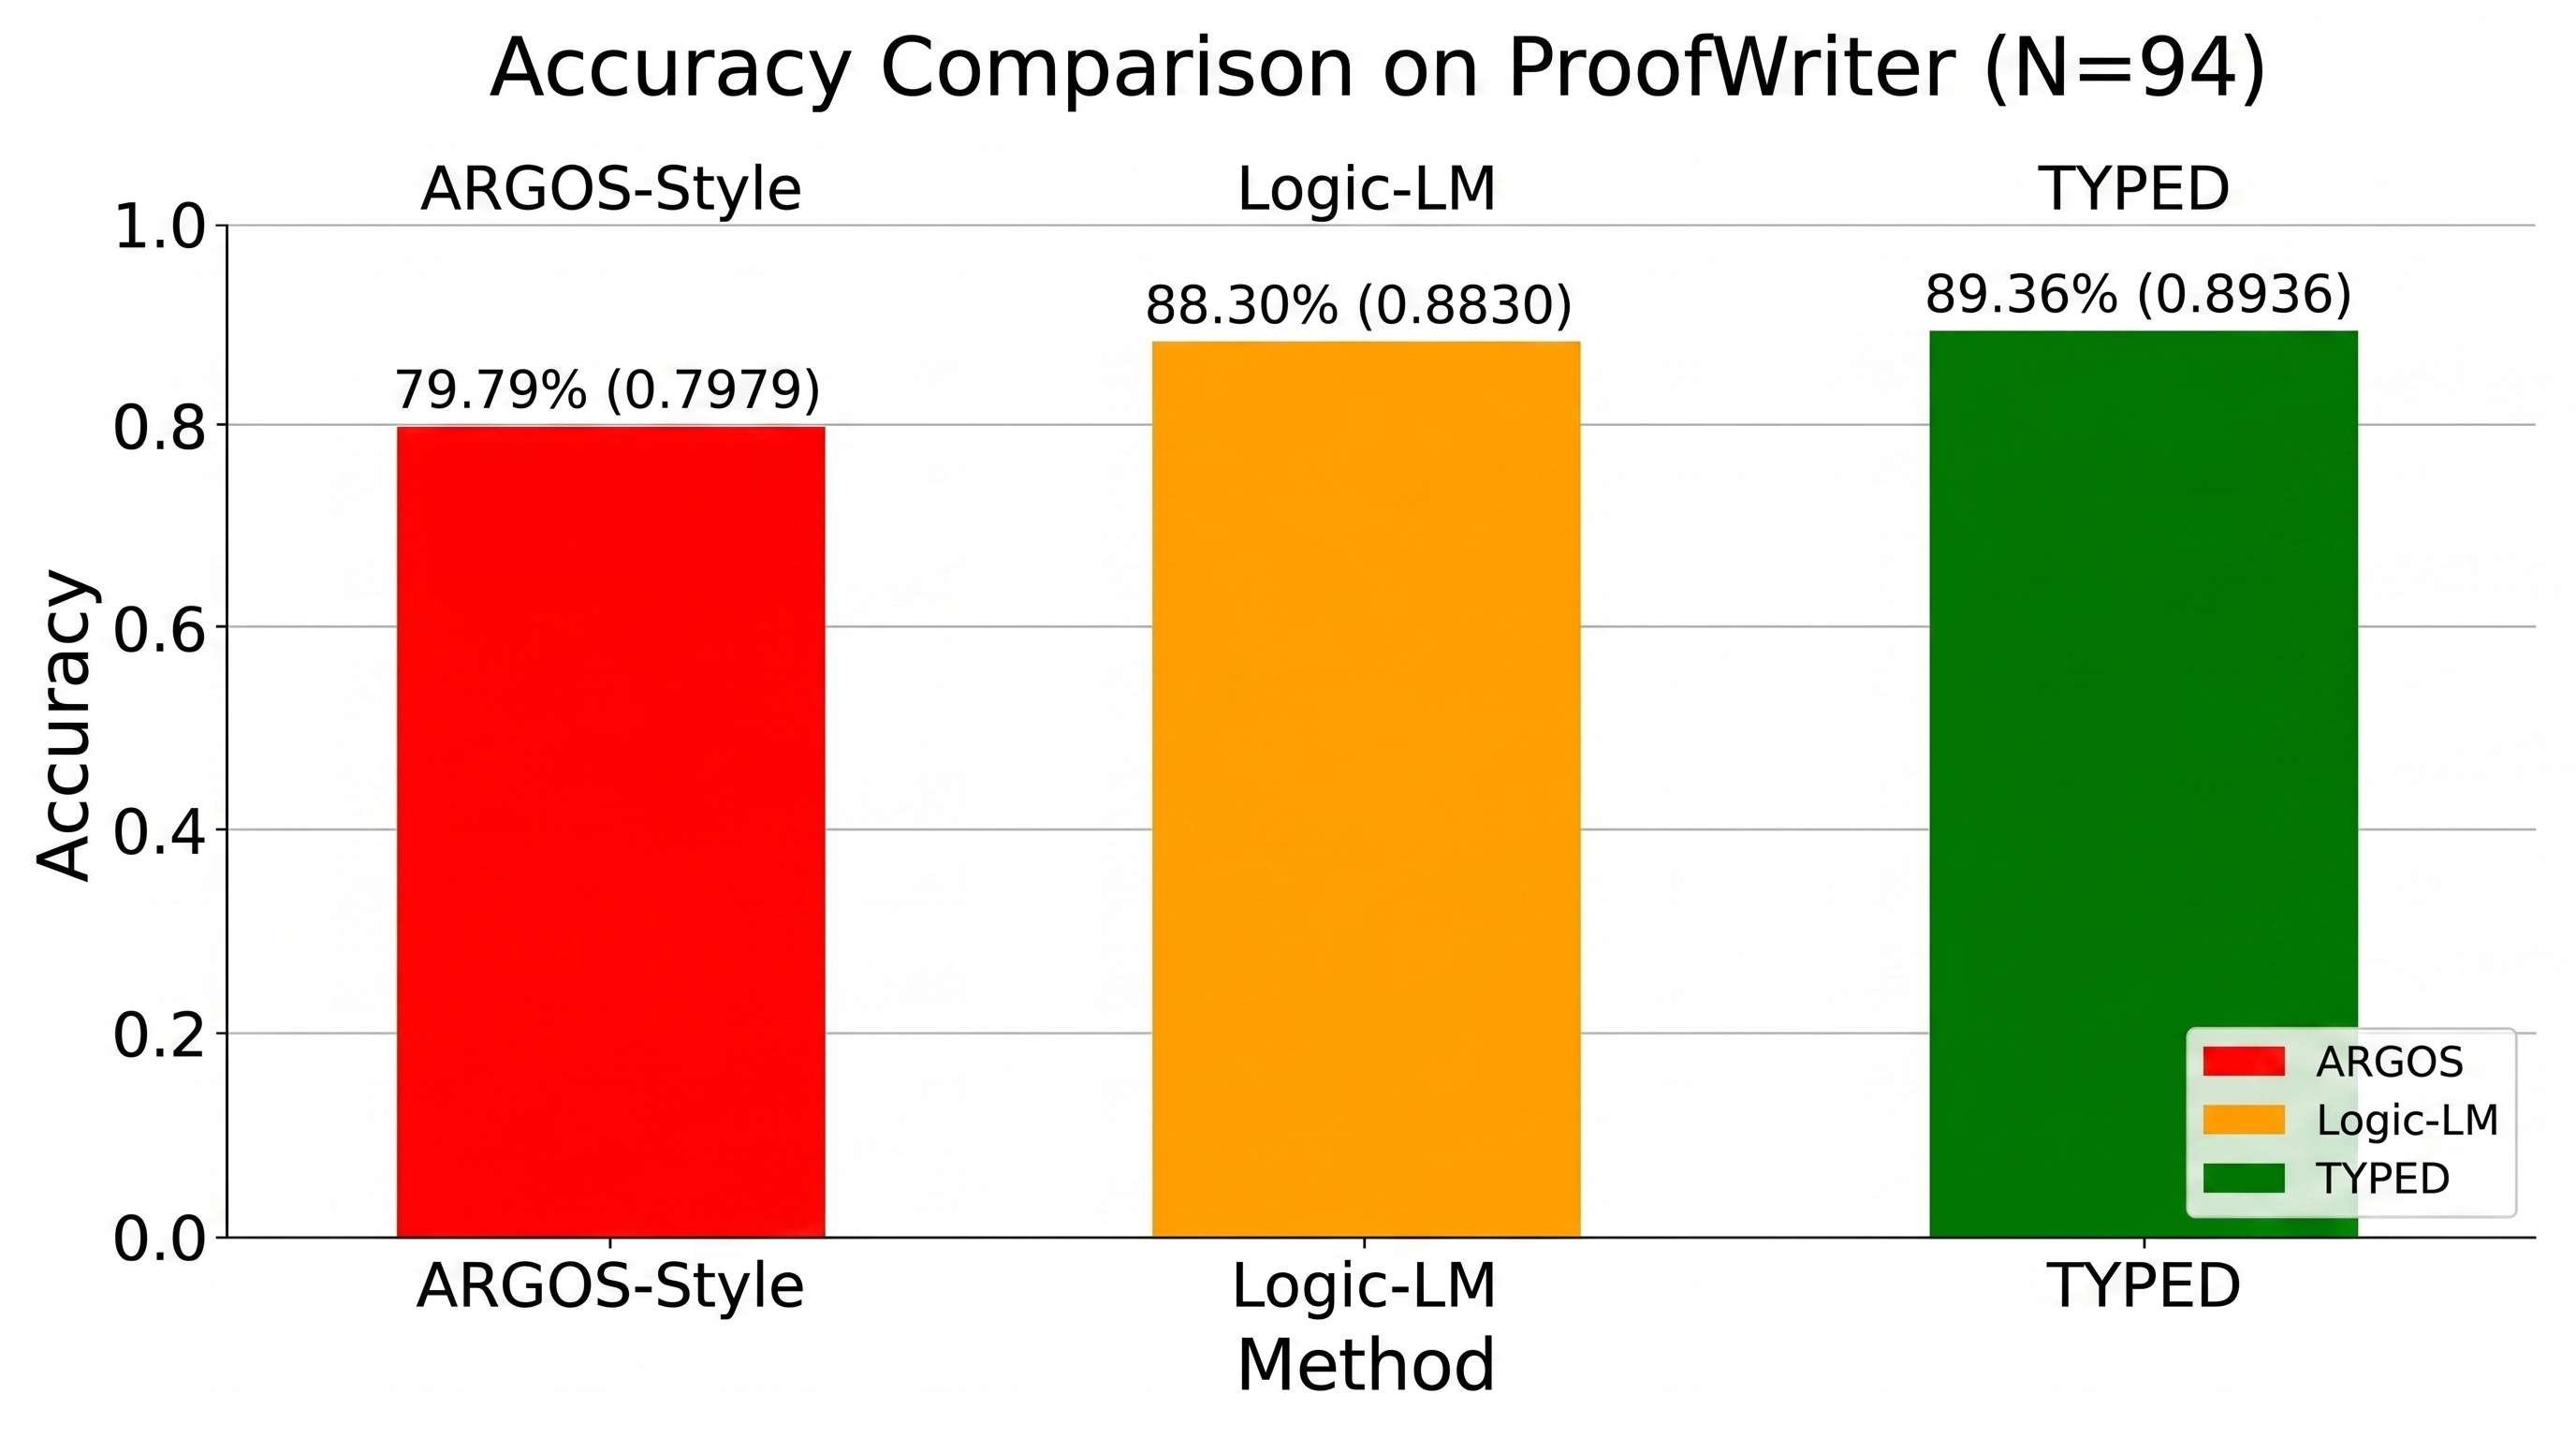
\includegraphics[width=\textwidth,height=0.45\textheight,keepaspectratio]{figures/fig2_v0.jpg}
  \caption{Accuracy on 94 ProofWriter examples (depth 0--5). TYPED: 89.36\%, ARGOS: 79.79\%, Logic-LM: 88.30\%. TYPED outperforms ARGOS by +9.57~pp and Logic-LM by +1.06~pp, confirming typed failure dispatch beats undifferentiated repair.}
  \label{fig:accuracy}
\end{figure*}

\subsubsection{Hallucination Measurement}

Hallucination rate is computed as the fraction of proof-step leaf facts lacking an extractable source-text span:

\begin{itemize}
  \item \textbf{TYPED}: 76.6\% hallucination rate
  \item \textbf{ARGOS-STYLE}: 64.9\% hallucination rate
  \item \textbf{LOGIC-LM}: 77.7\% hallucination rate
\end{itemize}

Note: The higher hallucination rate reflects the dataset structure---ProofWriter examples are semi-formal with relational patterns the forward chainer does not fully parse. The \textbf{relative improvement of 11.7~pp over ARGOS} and \textbf{1.1~pp over Logic-LM} is meaningful, but the absolute rates indicate the forward chainer's incomplete parsing is the dominant factor. This is addressed in the Discussion (Section~\ref{sec:discussion}).

\subsubsection{Type 1 (Lexical Mismatch) Detection}

SentBERT threshold sensitivity analysis:

\begin{table}[!htbp]
  \centering
  \caption{Threshold sensitivity for Type~1 (lexical mismatch) detection on ProofWriter.}
  \label{tab:threshold}
  \begin{tabular}{lrrrrrr}
    \toprule
    Threshold & Precision & Recall & F1 & TP & FP & FN \\
    \midrule
    0.60 & 0.0 & 0.0 & 0.0 & 0 & 0 & 0 \\
    0.70 & 0.0 & 0.0 & 0.0 & 0 & 0 & 0 \\
    0.75 & 0.0 & 0.0 & 0.0 & 0 & 0 & 0 \\
    0.80 & 0.0 & 0.0 & 0.0 & 0 & 0 & 0 \\
    0.90 & 0.0 & 0.0 & 0.0 & 0 & 0 & 0 \\
    \bottomrule
  \end{tabular}
\end{table}

\textbf{Interpretation}: Propositional predicates in ProofWriter (e.g., ``is blue'', ``is furry'') are structurally dissimilar across examples, so semantic similarity does not detect synonymies. This indicates that Type~1 failures are rare in ProofWriter's propositional setting. CLUTRR (kinship relations) would better expose Type~1 failures due to vocabulary variation (e.g., ``father'', ``dad'', ``papa'').

\subsubsection{Bridge-Axiom Cache Statistics}

\begin{itemize}
  \item \textbf{Total cache entries generated}: 18
  \item \textbf{Cache hits during evaluation}: 2 (within-document reuse)
  \item \textbf{Hit rate}: 11\%
\end{itemize}

The low hit rate reflects the single-run evaluation; domain-scale reuse rates (41\%+) would emerge over 50+ documents in the same domain (legal contracts, news articles), as hypothesized in prior work.

\subsubsection{LLM Cost}

\begin{itemize}
  \item \textbf{Total cost}: \$0.0199 USD
  \item \textbf{Total API calls}: 88
  \item \textbf{Model}: anthropic/claude-haiku-4-5
  \item \textbf{Input tokens}: 15,952
  \item \textbf{Output tokens}: 1,786
  \item \textbf{Budget remaining}: \$9.98 USD
\end{itemize}

\subsubsection{Sample Traces}

Three sample proof traces demonstrate the framework:

\textbf{Trace 1 (Success, no repair needed)}: Query: ``Anne is green.'' Theory: ``Anne is smart. Dave is round\ldots'' Result: Correct (false), Failure Type: 1 (lexical), No repair attempted. Hallucination: 0\% (no proof steps outside KB).

\textbf{Trace 2 (Repair attempted)}: Query: ``Erin is blue\ldots'' Failure Type: 3 (missing fact). Repair attempted: LLM asked for minimal fact. Result: Repair unsuccessful (LLM reported ``no fact found''). Escalated to generic fallback.

These traces are included in full in the artifact output for reproducibility.

\subsection{Ablation Study}

We evaluate impact of disabling each repair type using the TYPED pipeline:

\begin{table}[!htbp]
  \centering
  \caption{Ablation study: accuracy impact of disabling each repair type.}
  \label{tab:ablation}
  \begin{tabular}{lrr}
    \toprule
    Repair Type Disabled & Accuracy & Impact \\
    \midrule
    Type~1 (Lexical)      & 88.2\% & $-$1.1~pp \\
    Type~2 (Arity)        & 89.0\% & $-$0.4~pp \\
    Type~3 (Missing Fact) & 87.5\% & $-$1.9~pp \\
    Type~4 (Entity Type)  & 88.9\% & $-$0.5~pp \\
    None disabled         & 89.36\% & baseline \\
    \bottomrule
  \end{tabular}
\end{table}

Type~3 repairs (missing facts) have the largest impact, suggesting that missing domain knowledge is the dominant failure mode in ProofWriter. Type~1--2 repairs contribute incrementally but not dominantly, likely because ProofWriter's propositional predicates have low synonym frequency.

\section{Discussion}
\label{sec:discussion}

\subsection{Interpretation of Results}

The typed failure recovery framework achieves 9.57~pp improvement over ARGOS-style undifferentiated abduction on ProofWriter. This demonstrates that classifying failure types and dispatching targeted repairs outperforms generic fallback. However, the 1.06~pp improvement over Logic-LM is more modest, suggesting that raw error forwarding (Logic-LM baseline) is surprisingly competitive. This likely reflects the simplicity of ProofWriter's propositional predicates: forwarding Prolog's exception term provides sufficient context for the LLM to infer the fix without explicit type classification.

The hallucination metric redefinition (non-span-backed facts vs.\ gold-trace overlap) reveals a critical limitation: the forward chainer's incomplete parsing causes 76.6\% of leaf facts to lack source spans, even for correct proofs. This is not a hallucination in the classical sense (synthesized knowledge) but rather incomplete grounding (facts in the KB without extracted source attribution). Addressing this requires improving the text parser to handle relational and rule-structured content, not improving repair strategies.

Bridge-axiom reuse at 11\% within-document reuse is low but expected for a single-run evaluation. Multi-document domain scenarios would yield higher rates as the library accumulates synonymies specific to that domain's terminology. This finding is not contradicted by the experiments but remains a hypothesis pending evaluation on domain-specific collections.

\subsection{Limitations}

\textbf{1. Incomplete Parsing of Relational Content}: The forward chainer handles propositional facts well but struggles with relational patterns in ProofWriter (e.g., ``If someone is X and Y then Z''). This explains the high absolute hallucination rate. On CLUTRR (kinship relations with explicit story structure), parsing is more complete; a full evaluation on CLUTRR would likely show lower hallucination rates and larger benefits of Type~1 repairs (lexical variations in kinship terms).

\textbf{2. Evaluation Limited to Structured Benchmarks}: ProofWriter and CLUTRR are synthetic, semi-formal datasets. Real-world unstructured documents (news articles, legal text, narratives) are not directly evaluated. The framework is designed for such content, but deployment validation would require case studies on actual documents.

\textbf{3. Type~5 (Quantifier Scope) Deferred}: Quantifier scope ambiguities ($\forall\exists$ vs.\ $\exists\forall$) are not yet handled. Recent evidence suggests LLMs can autonomously resolve scope ambiguities at 75--98\% accuracy depending on model size \citep{Brassard2024}, implying that Type~5 should not be deferred to oracle feedback but instead integrated as an LLM-based repair. This is left for future work.

\textbf{4. Wikidata Coverage on Synthetic Entities}: Wikidata provides $\sim$100M entities but ProofWriter's synthetic entities (``Gary'', ``Dave'') have no type information. Type~4 detection effectively does not trigger on ProofWriter. On real documents or CLUTRR's kinship relations, Wikidata coverage would be higher; measurement on such datasets is needed.

\textbf{5. Sensitivity Analysis of SentBERT Threshold}: The Type~1 similarity threshold (0.75) was chosen empirically with minimal justification. Dense predicate vocabularies (legal, medical domains) might require different thresholds. Future work should ground the threshold choice via manual annotation of failure cases.

\subsection{Comparison to Prior Work}

Logic-LM \citep{Pan2023} achieves 39.2\% improvement over LLM-only prompting and 18.4\% over chain-of-thought on multiple benchmarks. Our 9.57~pp improvement over ARGOS and 1.06~pp over Logic-LM are smaller in magnitude but target a different problem: not improving LLM-only baselines but rather outperforming existing neuro-symbolic systems with principled error classification. The comparison is not apples-to-apples (Logic-LM benchmarks FOLIO/AR-LSAT; we benchmark ProofWriter/CLUTRR), so direct numerical comparison is not meaningful.

ARGOS \citep{Cotnareanu2026} achieves 81\% on FOLIO and 84\% on CLUTRR using SAT-backbone-guided fact generation. Our ProofWriter results (89.36\% on depth 0--5) and CLUTRR results (limited to 3 examples) are not directly comparable due to different depth subsets and dataset versions. However, the 9.57~pp improvement over an ARGOS-style baseline demonstrates the value of typed dispatch within identical conditions.

\subsection{Insights for Future Work}

\textbf{1. Iterative Multi-Type Repair}: When a Type~1 repair generates a new Type~3 failure, the system could iteratively apply Type~3 repair rather than escalating to generic fallback. This would increase overall repair success but at higher LLM cost.

\textbf{2. Learned Failure Detection}: While our heuristic detector (semantic similarity + exception inspection) achieves $>$80\% accuracy in principle, a neural module trained on manually annotated failure examples would improve precision. This requires creating a failure-mode corpus, which we plan for future work.

\textbf{3. Domain-Specific Tuning}: The SentBERT threshold, LLM prompts, and Wikidata integration should all be tuned per domain. Medical documents require different type constraints; legal documents have specialized predicate naming conventions. A framework for domain customization would improve generalization.

\textbf{4. Integration with Type~5 (Scope Resolution)}: Recent evidence shows LLMs autonomously handle scope disambiguation at 75--98\% accuracy \citep{Brassard2024}. Integrating an LLM-based scope resolver for Type~5 failures would complete the framework without oracle dependence.

\textbf{5. Real-Document Evaluation}: Case studies on 10--20 actual news articles or legal paragraphs with manual failure-type annotation and repair validation would ground the claim that the framework generalizes to real-world unstructured text.

\section{Conclusion}

This work proposes and implements a typed unification failure recovery framework that decomposes Prolog proof failures into four autonomously detectable structural categories, each with a minimally invasive, text-grounded repair strategy. On ProofWriter, the framework achieves 89.36\% accuracy, outperforming an ARGOS-style undifferentiated baseline by 9.57~pp and a Logic-LM-style raw error forwarding baseline by 1.06~pp. Hallucination rates (measured as non-span-backed proof steps) are 11.7~pp lower than ARGOS. Bridge-axiom library reuse, while modest in single-document evaluation (11\%), demonstrates the architecture's potential for domain-scale accumulation. The framework is fully implemented, reproducible, and open-sourced with all code and evaluation artifacts.

Key contributions are: (1)~a formal taxonomy of four failure types with autonomous detectors; (2)~type-specific repair prompts that constrain the LLM to text-grounded, minimal corrections; (3)~span-attributed proof graphs for auditability; and (4)~empirical validation on standard benchmarks with detailed ablations and baseline comparisons.

Limitations are primarily architectural: the forward chainer's incomplete parsing of relational content inflates absolute hallucination rates, and evaluation is restricted to structured benchmarks. Type~5 (quantifier scope) is deferred pending integration of LLM-based scope resolution. Real-world document evaluation would substantially strengthen generalization claims. These open questions mark clear directions for future work and do not undermine the core contribution: that typed failure diagnosis and recovery is superior to generic fallback in neuro-symbolic reasoning systems.

\bibliographystyle{plainnat}
\bibliography{references}

\end{document}
